\setboolean{IsHalfPage}{false}%
\setboolean{IsHalfPageLeftCol}{false}%
\setboolean{IsHalfPageRightCol}{false}%
\def\ChapterTitle{%
	Rattan Charm
}
\def\ChapterUrl{%
	https://arnottferels.github.io/work/rattan-charm
}
\def\ChapterDescription{%
	Redefining the Bedroom in BSD House with Full Ceiling Weave
}
\def\ChapterDetailsLine{%
	Professional Work -- 2021 | Rattan, Pattern Generation; Design | BSD, Indonesia
}
\def\ChapterDetailsTabular{%
	\begin{tabular}{@{}ll}
		\textbf{Contributions} & Research and Development, Conceptual Design, Digital Modeling \& Scripting \\
		\textbf{Software}      & Rhino \& Grasshopper                                                       \\
		\textbf{Team Leader}   & Trianzani Sulshi                                                           \\
		\textbf{URL}           & \textcolor{blue}{\footnotesize\texttt{\href{\ChapterUrl}{\ChapterUrl}}}    \\
	\end{tabular}
}
\def\ChapterAbstract{%
	This project delves into two design options: Pyramid and Wave Rattan pattern generation. The Pyramid approach involves systematically creating intricate two-dimensional patterns, refining them in the third dimension using weaving techniques, thereby enhancing the understanding of multidimensional pattern manipulation. The Wave design introduces a rattan object shaped like a flag for the ceiling, fulfilling the client's need for visibility from diverse angles, particularly from the bed. This addition contributes a dynamic and visually appealing element to the overall space.
}
\def\ChapterFrontmatter{%
	\chapter*{\ChapterTitle}\addcontentsline{toc}{chapter}{\ChapterTitle}
	\ChapterSetTocAddData{\ChapterDetailsLine}
	\ChapterSetDetailsData{\ChapterDescription}{\ChapterDetailsLine}{\ChapterDetailsTabular}
	\RuleAbstract%
	\ChapterAbstract
}
\StartTwoColumnLayout
\ChapterFrontmatter
\section*{
  Inspiration \& Pattern Generation
 }
\vspace{-\baselineskip}%
\setlength{\columnsep}{0.25cm}%
\begin{multicols}{2}
	\subsection*{
		Option 1: Pyramid
	}
	%
\begin{figure}[H]
	\centering
	\includesvg[width=\linewidth]{src/graphics/rattan-charm--inspiration-opt-01-pyramid.svg}
	\label{
		fig:rattan-charm--inspiration-opt-01-pyramid
	}
\end{figure}

	\vfill
	%
\begin{figure}[H]
	\centering
	\includesvg[width=\linewidth]{src/graphics/rattan-charm--pattern-generation-opt-01-pyramid.svg}
	\label{
		fig:rattan-charm--pattern-generation-opt-01-pyramid
	}
\end{figure}

	\vspace{0.125cm}%
	In Option 1 Pyramid Design, systematic iterations produced intricate 2D patterns extended into the third dimension (Z-coordinate). Weaving methods like (0-1-1-0) and (0-1-0-1) enhanced pattern manipulation across multiple dimensions.
	\vspace*{\baselineskip}
	%
\begin{figure}[H]
	\centering
	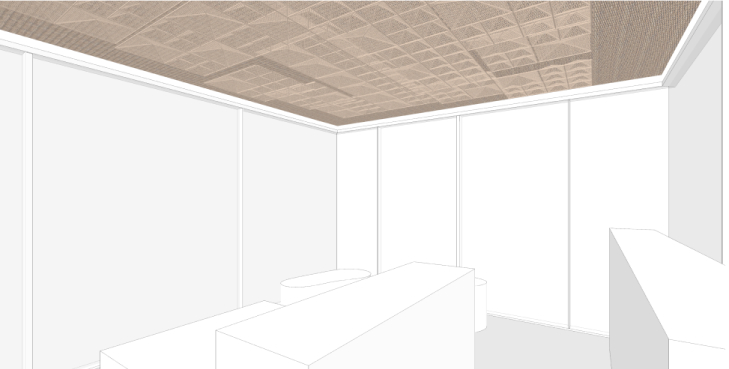
\includegraphics[width=\linewidth]{src/graphics/rattan-charm--pattern-generation-opt-01-pyramid-perspective.jpg}
	\caption*{%
		Option 1: Pyramid
	}
	\label{
		fig:rattan-charm--pattern-generation-opt-01-pyramid-perspective
	}
\end{figure}

	\columnbreak%
	\subsection*{
		Option 2: Wave
	}
	%
\begin{figure}[H]
	\centering
	\includesvg[width=\linewidth]{src/graphics/rattan-charm--inspiration-opt-02-wave.svg}
	\label{
		fig:rattan-charm--inspiration-opt-02-wave
	}
\end{figure}

	\vfill
	%
\begin{figure}[H]
	\centering
	\includesvg[width=\linewidth]{src/graphics/rattan-charm--pattern-generation-opt-02-wave.svg}
	\label{
		fig:rattan-charm--pattern-generation-opt-02-wave
	}
\end{figure}

	\vspace{0.125cm}%
	In Option 2 Wave Design, a rattan object resembling a flag acts as an elegant ceiling ornament. The client's request for visibility, especially from the bed, enhances the space with a dynamic and visually appealing element.
	\vspace*{\baselineskip}
	%
\begin{figure}[H]
	\centering
	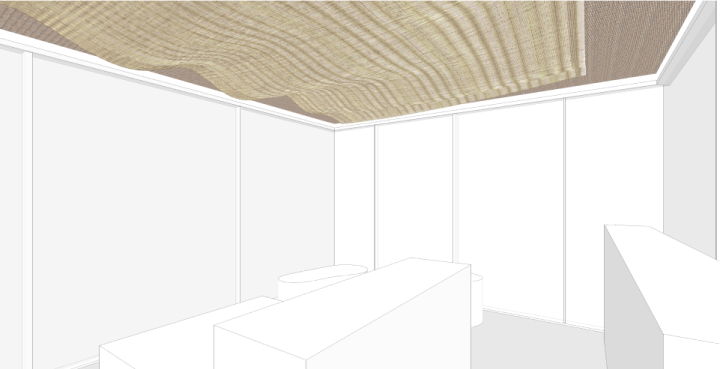
\includegraphics[width=\linewidth]{src/graphics/rattan-charm--pattern-generation-opt-02-wave-perspective.jpg}
	\caption*{%
		Option 2: Wave
	}
	\label{
		fig:rattan-charm--pattern-generation-opt-02-wave-perspective
	}
\end{figure}

\end{multicols}
\columnbreak%
\begin{minipage}[t][\textheight][t]{\linewidth}
	\section*{
	  Design \& Details
	 }
	\vspace{-\baselineskip}%
	\subsection*{
		Option 1: Pyramid
	}
	\makebox[\linewidth][l]{%
		\hspace{\linewidth-0.95\linewidth}
		\begin{minipage}{0.95\linewidth}
			\vspace{-\baselineskip}%
			\noindent
			%
\ImageWidth=\dimexpr(\linewidth)\relax
\def\FigureRattanCharmDesignDetailsOptOnePerspective{%
	\includesvg[width=\linewidth]{src/graphics/rattan-charm--design-details-opt-01-pyramid.svg}
}
\def\Figure{\FigureRattanCharmDesignDetailsOptOnePerspective}
\settototalheight{\ContentHeight}{\Figure}
\begin{figure}[H]
	\centering
	\begin{minipage}{\linewidth}
		\FigureRattanCharmDesignDetailsOptOnePerspective
		\begin{picture}(0,0)
			\put(0.7\ImageWidth,0.1\ContentHeight){%
				\parbox{0.3\ImageWidth
					-3pt%
				}{%
					\raggedright
					{%
						\textnormal{%
							\footnotesize
							Based on the iterations conducted, the axonometric design of Option 1 Pyramid is composed of several $\textnormal{4} \times \textnormal{6}$ panels, totaling 24~panels arranged diagonally.
						}
					}
				}
			}
		\end{picture}
	\end{minipage}
	\label{
		fig:rattan-charm--design-details-opt-01-pyramid
	}
\end{figure}

		\end{minipage}
	}
	\vfill
	\subsection*{
		Option 2: Wave
	}
	\makebox[\linewidth][l]{%
		\hspace{\linewidth-0.95\linewidth}
		\begin{minipage}{0.95\linewidth}
			\vspace{-\baselineskip}%
			\noindent
			%
\ImageWidth=\dimexpr(\linewidth)\relax
\def\FigureRattanCharmDesignDetailsOptTwoPerspective{%
	\includesvg[width=\linewidth]{src/graphics/rattan-charm--design-details-opt-02-wave.svg}
}
\def\Figure{\FigureRattanCharmDesignDetailsOptTwoPerspective}
\settototalheight{\ContentHeight}{\Figure}
\begin{figure}[H]
	\centering
	\begin{minipage}{\linewidth}
		\FigureRattanCharmDesignDetailsOptTwoPerspective
		\begin{picture}(0,0)
			\put(0.7\ImageWidth,0.1\ContentHeight){%
				\parbox{0.3\ImageWidth
					-3pt%
				}{%
					\raggedright
					{%
						\textnormal{%
							\footnotesize
							Based on the iterations conducted, the design of Option 2 Wave consists of 3 elongated panels locked along their length.
						}
					}
				}
			}
		\end{picture}
	\end{minipage}
	\label{
		fig:rattan-charm--design-details-opt-02-wave
	}
\end{figure}

		\end{minipage}
	}
\end{minipage}
\EndTwoColumnLayout
\newpage
